\documentclass{article}
\usepackage[utf8]{inputenc}
\usepackage{amsmath}
\usepackage{listings}
\usepackage{geometry}
\usepackage{graphicx}
\usepackage{appendix}
\usepackage{subfig}
\usepackage{gensymb}
\usepackage{cancel}
\usepackage{physics}
\usepackage[colorlinks=true]{hyperref}
\usepackage{xcolor}
\definecolor{codegreen}{rgb}{0,0.6,0}
\definecolor{codegray}{rgb}{0.5,0.5,0.5}
\definecolor{codepurple}{rgb}{0.58,0,0.82}
\definecolor{backcolour}{rgb}{0.95,0.95,0.92}
\lstdefinestyle{mystyle}{
    backgroundcolor=\color{backcolour},   
    commentstyle=\color{codegreen},
    keywordstyle=\color{magenta},
    numberstyle=\tiny\color{codegray},
    stringstyle=\color{codepurple},
    basicstyle=\ttfamily\footnotesize,
    breakatwhitespace=false,         
    breaklines=true,                 
    captionpos=b,                    
    keepspaces=true,                 
    numbers=left,                    
    numbersep=5pt,                  
    showspaces=false,                
    showstringspaces=false,
    showtabs=false,                  
    tabsize=2
}

\lstset{style=mystyle}

\title{%
Project 5 - Social Ising Model\\
\large Using a Social Ising Model to model a binary election \\
\large in a closed community \\
\large FYS3150 at University of Oslo}
\author{Simen Løken}
\date{December 2020}
\footskip = 90pt
\topmargin = -40pt

\begin{document}

\maketitle
{
  \hypersetup{linkcolor=black}
  \tableofcontents
}
\newpage
\section{Abstract}
In this report, we'll examine how to use a simple chain/one dimensional Ising spin model to describe the opinion dynamics of a closed community. We do this via using a Monte Carlo simulation, and we find both a successful model and a relationship between the decision times of the model and a power law with exponent $-3/2$. Lastly, we also find that for a closed community, there will always be (given enough time) either a consensus A, B or a complete stalemate, never any in between. To avoid this, we find that an "openness" of $p \geq 3\times 10^{-5}$ is needed to avoid a "one-party state".
\section{Introduction}
The concept of a social Ising model, alternatively the Sznajd model was first proposed by the married couple Sznajd in 2000 \cite{sznajd}, as an attempt at using the statistical method of a one dimensional Ising model to model opinion dynamics in a closed community. The model has since been accepted as a useful tool for modeling the social dynamics with a binary outcome, although limited, and can be used to give useful insight into how opinions may develop and spread.\newline
While relatively simple in scale, the model is surprisingly useful in simulating real life opinion dynamics. Although limited to a binary output, we don't necessarily need to model, say a two candidate election, but could instead apply the model to a yes or no question, or any kind of vote with only two outcomes. It is therefore that this model is so interesting and why we wish to study it in this article.\newline
In this article we're going to first be modelling a system like this from the ground up, before later applying the model so we if we can replicate the results from \cite{sznajd}, within a tolerance. Note that because of the random nature of this model (every run is unique), we can't expect identical results, but we should see the same tendencies. We're going to study the model in itself, through a combination of studying the magnetization, the auto correlation and see if we can find a relationship between the decision time and a power law logarithmicly, before then examining the effect of a noise, and how much effect it can have on the model. Lastly, we'll discuss our results and compare them to the ones found in \cite{sznajd}.
\section{Theory}
Recall \cite{proj4} that the energy of an Ising model can be expressed as:
\begin{equation*}
    E = - J \sum_{\langle kl \rangle}^N s_k s_i
\end{equation*}
It follows then naturally that the magnetization of such a system can be expressed as:
\begin{equation}
    m = \frac{1}{N} \sum_{i=1}^N S_i
\end{equation}
where $N$ is the total number of elements in the chain and $S_i$ is the spin of the element $i$. \newline
We can also study the time correlation of m using the classical autocorrelation function:
\begin{equation}
    G(\Delta t) = \frac{\sum (m(t) - \langle m \rangle)/m(t+ \Delta t) - \langle m \rangle}{\sum (m(t) - \langle m \rangle)^2}
\end{equation}
\newpage
\section{Method}
\subsection{The One Dimensional Ising Model}
We've already discussed the two dimensional Ising Model in the previous project 4 \cite{proj4}, but let us quickly recap. \newline
The Ising model is primarily a model for modelling the spin of particles. Recall that there are only two possible values of spin, thus we get a binary model. \newline
While for the two dimensional model, we picked a random point, or spin, and examined it with its neighbour to get one of four possible states. The one dimensional method is much the same, but we instead have a chain of random points, or spins. We then select a random point and instead examine the two closest neighbours on the chain.
\subsection{The Rules}
In order for this to properly model social pressure and an election, we need to make a few rules as to how our model should behave. \newline
Let us then define the following rules: \newline
For a given time step, assume we pick a random spin, or point on the chain $S_i$.
\begin{itemize}
    \item If $S_i = S_{i+1}$\newline
    then:
    \begin{itemize}
        \item $S_{i-1} = S_i$ and $S_{i+2} = S_i$
    \end{itemize}
    \item If $S_i \neq S_{i+1}$ or rather, $S_i = -S_{i+1}$\newline
    then:
    \begin{itemize}
        \item $S_{i-1} = S_{i+1}$ and $S_{i+2} = S_i$
    \end{itemize}
\end{itemize}
This may initially seem like a random, or perhaps arbitrary definition of our model, but the idea is two basic principles. \newline
The model is founded in the ideas of \textbf{Social Validation} and \textbf{Discord Destroys}, so essentially what we're looking at is if two people ($S_i$ and $S_{i+1}$) share an opinion, then their adjacent neighbours will agree with them in turn (Social Validation), however, if two people disagree, then their neighbours will argue (Discord Destroys). As a visual aid for understanding this model, refer to the below image [\ref{fig1}].
\begin{figure}[ht!]
    \centering
    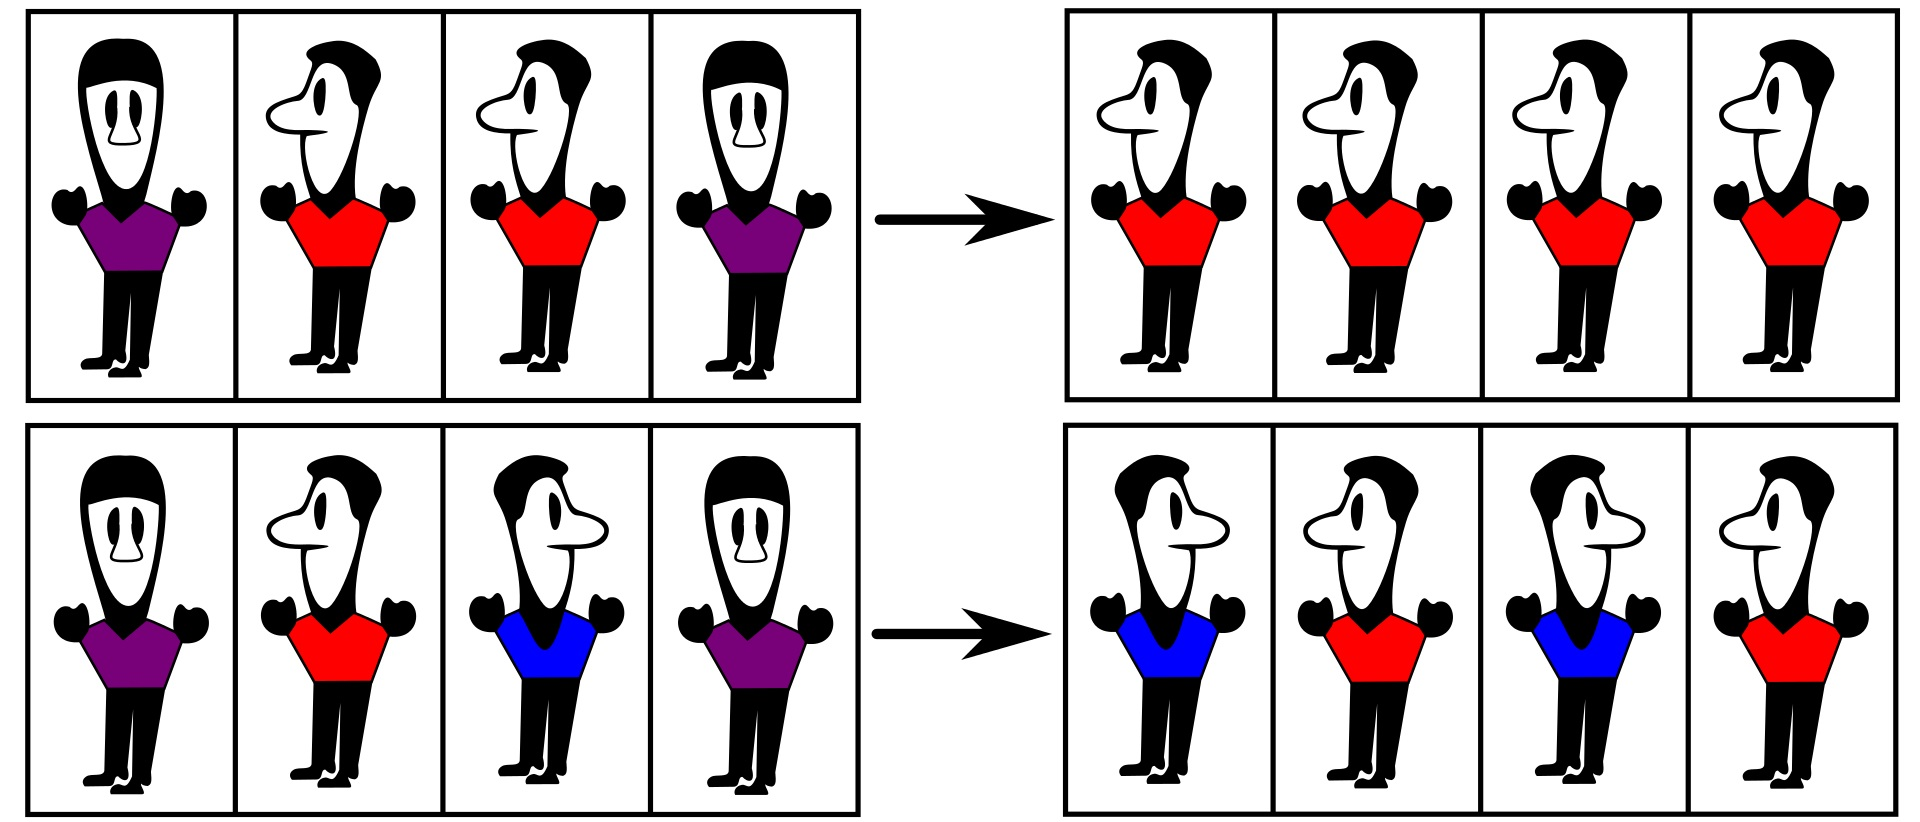
\includegraphics[scale=0.2]{modelIllustrated.jpg}
    \caption{An illustration showing the two cases of our model. \newline
    Although this wouldn't actually happen in our model (our model is binary), assume for simplicity's sake that the purple men are undecided, whilst red is for and blue is against. \newline
    In the uppermost case, we have  \textbf{Social Validation}, and everyone agrees, while in the lowermost case, we have a disagreement, thus leading to all neighbours disagreeing with each other, \textbf{Discord Destroys}. \newline
    Illustration retrieved from \cite{sznajdwiki}}
    \label{fig1}
\end{figure}
\newpage
\subsection{Modelling an election}
We will use the model described above to model some kind of binary problem, a problem where there are only two possible outcomes. Whether we decide to call this a for/against model or a two-party election model does not matter in the grand scheme of things, but in light of recent happenings, let us assume it is an election in a two-party state. \newline
We will then assume that it is of course not possible to abstain from voting. We should then as our model stabilizes after a sufficient number of Monte Carlo cycles, reach one of three states:
\begin{itemize}
    \item Candidate A wins
    \item Candidate B wins
    \item Stalemate
\end{itemize}
Of course, were we to stop the simulation early before any sort of consensus were reached, we'd find the population leaning towards one candidate, but no consensus reached.
\newline This could, somewhat on the nose,  perhaps be described as a one-party state, or rather, a "monopoly" on politics for either candidate A or B, while for stalemate the population is unable to reach a decision. This is the result of our "closed community". To try and remedy this, we will later on in our model add a new factor, where we can add a random chance that a given spin will flip from outward influence. To help with imagining this in a real life scenario, think of this as the internet or rather an open community.
\newpage
\section{Results}
Let first examine a typical evolution of opinions over a set number of Monte Carlo cycles. We're going to be using a total of spins:
\begin{figure}[ht!]
    \centering
    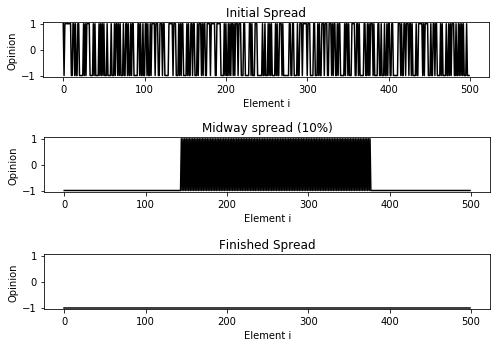
\includegraphics[scale=0.7]{evolution.png}
    \caption{First the initial spread of opinions, then the a snapshot taken at 1 000 000 MCS. Finally, we have the finished opinion spread at about ~ 2 000 000 MCS }
    \label{fig2}
\end{figure} \newline
Note that when the actual convergence/consensus is reached is different for each iteration of the program. In this case, we let the program run for a total of 10 000 000 MCS, and take a snapshot at every 10\%. This saves significantly on computation time (because once a consensus is reached, the state is unchanging). \newline
Let us now for this same run examine the magnetization:
\begin{figure}[ht!]
    \centering
    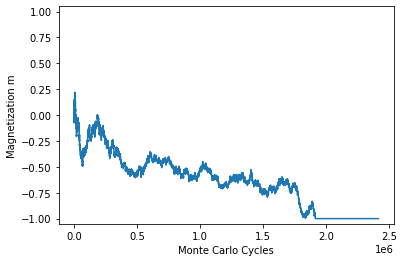
\includegraphics[scale=0.6]{magnetization.png}
    \caption{The magnetization over time. \newline
    As expected, it settles at -1, which was the consensus reach above in figure [\ref{fig2}]}
    \label{fig3}
\end{figure} \newline
As expected, we see much the same behavior as the ones in the Sznajd paper, except theirs stabilized at a value $m = 0$, meaning a stalemate, whereas ours stabilized at $m = -1$, meaning candidate B in our case.
\newline
Let us now examine the same set of results through the autocorrelation function:
\begin{figure}[ht!]
    \centering
    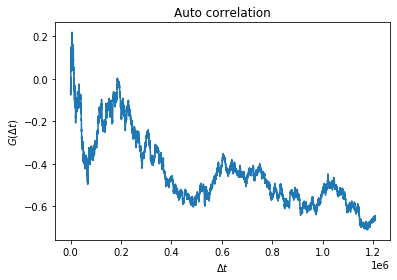
\includegraphics[scale=0.6]{autocorrelation.png}
    \caption{The autocorrelation over time. \newline
    Keep in mind that this is probably off, I couldn't get the auto correlation to work (I think).}
    \label{fig4}
\end{figure} \newline
Here we see a measurement for how likely a given spin is to change its opinion, which we see is very likely. \newline
Let us now try to correlate the decision times observed against a power law, as done in the Sznajd paper.
We get:
\begin{figure}[ht!]
    \centering
    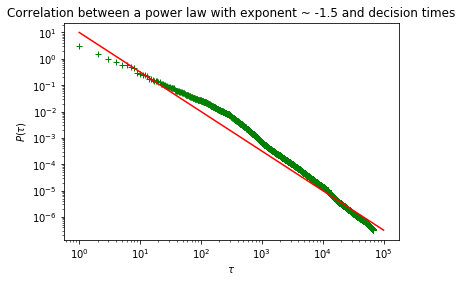
\includegraphics[scale=0.55]{decisiontimes.png}
    \caption{The decision times. \newline
    As expected, we see (but perhaps not as clearly), that there is a significant increase in density of points as we go along the x-axis. This is in line with the results in Sznajd's paper, that the decision times are generally very short.}
    \label{fig4}
\end{figure} \newpage
We see here that the density increases greatly for points of shorter decision times, as expected. We see also that it follows the power law of $-3/2$, also as expected. This tells us that we were correct in our assumption above, that a lot of decision times are small, or that a given spin is likely to change its opinion often.
\newline
Let us now instead examine the effects of selecting a certain percentage of the population to have opinion B. We let this percentage be 20\% and try for a random configuration:
\begin{figure}[ht!] 
\centering
\subfloat[Magnetization]{
  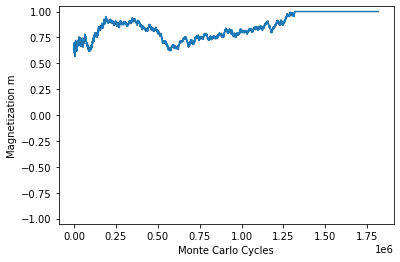
\includegraphics[width=65mm]{magnetizationB20.png}
}
\subfloat[Decision Times]{
  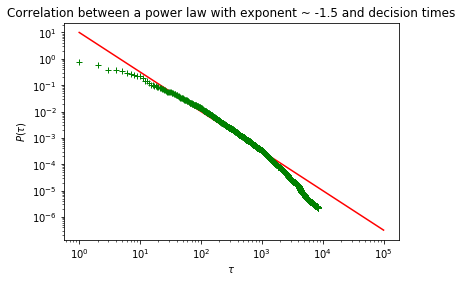
\includegraphics[width=65mm]{decisiontimesB20.png}
}
\caption{Here we see the magnetization of our model with an initial random population of 20\% B. \newline
You might notice that the magnetization is not 0.8, which it should be if B = 0.2. This is because the first sampling of m happens after a Monte Carlo cycle, so that's my bad. \newline
Additionally we see that the decision times no longer follow the $-3/2$ power law as closely. \newline
Note also that we (as expected) reach an A consensus when the population of B's are so small, though this does not always happen.}
\end{figure} \newline
Let us now examine the same, but for a clustered initial spread:
\begin{figure}[ht!] 
\centering
\subfloat[Magnetization]{
  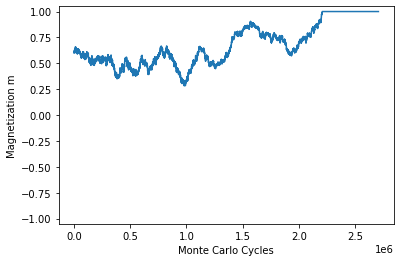
\includegraphics[width=65mm]{magnetizationB20clustered.png}
}
\subfloat[Decision Times]{
  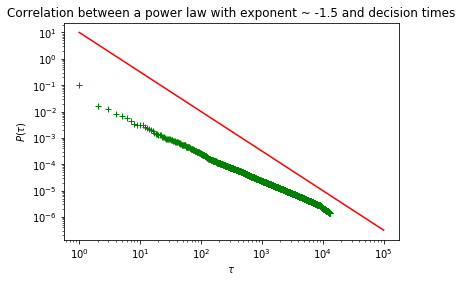
\includegraphics[width=65mm]{decisiontimesB20clustered.png}
}
\caption{Here we see the magnetization of our model with an initial clustered population of 20\% B. \newline
Here we also reach an A consensus as above.\newline
Additionally we see that the decision times no longer even remotely follow the $-3/2$ power law.}
\end{figure} \newline
We see above that as perhaps expected, we more commonly reach an A consensus than a B consensus (or stalemate) when the population of B is so tiny. It is however very important to stress that as the model is in its entirety random, there is still a very real chance of reaching both a B and a stalemate consensus. \newline
Note that there is no substantial difference between the results outside of the power law. That is, the chances of reaching an A, B or stalemate consensus is practically (within reason, since the random placement is just that, random) the same. It might be tempting to believe that a clustered configuration is more likely, given that you've got all opinion B's in one place, but this is not the case since the model in its very nature is random. This is also mentioned in Sznajd's paper.
\newline
Let us now examine how our model can handle a noise. For the purposes of the model, let this noise be the probability that a random element $i$ switches opinion at a given timestep. \newline We then get the plots:
\begin{figure}[ht!] 
\centering
\subfloat[p = $3 \times 10^{-6}$]{
  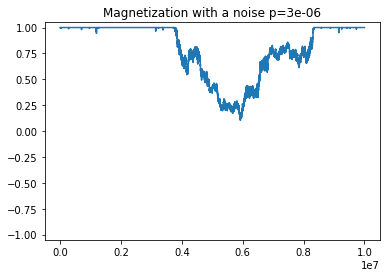
\includegraphics[width=55mm]{magnetNoise_3e-6.png} \label{fig5a}
}
\subfloat[p = $3 \times 10^{-5}$]{
  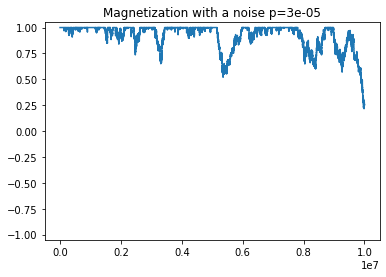
\includegraphics[width=55mm]{magnetNoise_3e-5.png} \label{fig5b}
}
\newline
\subfloat[p = $3 \times 10^{-4}$]{
  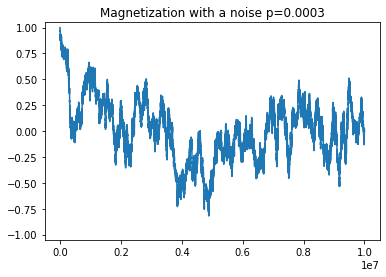
\includegraphics[width=55mm]{magnetNoise_3e-4.png} \label{fig5c}
}
\subfloat[p = $3 \times 10^{-6}$]{
  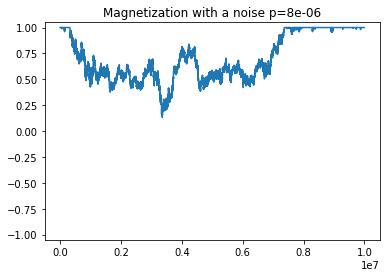
\includegraphics[width=55mm]{magnetNoise_8e-6.png} \label{fig5d}
}
\caption{Here we see the magnetization for different probabilities $p$. \newline
In the case of figure [\ref{fig5a}], we see that although the probability can somewhat shake our system out of order, it is still able to correct itself and stabilize.
\newline In the case of figure [\ref{fig5b}], we see that it is oscillating between an ordered and an unordered state. It would perhaps be natural, based on this behavior, to assume this to be the limit between an ordered and an unordered state.
\newline For figure [\ref{fig5c}], we see that we are incredibly unordered. This probability is way too high and likely has no chance to recover.
\newline Lastly to further reinforce what was mentioned for figure [\ref{fig5b}], we see that for figure [\ref{fig5d}], it is still able to recover despite being closer to $3\times 10^{-5}$ than figure [\ref{fig5a}]}
\end{figure} \newpage
The results above are indicative of a certain degree of "openness" that is required to keep the closed community from becoming a one-party state, or alternatively a dictatorship. \newline
Lastly, let us examine the decision times for different probabilities $p$:
\begin{figure}[ht!]
    \centering
    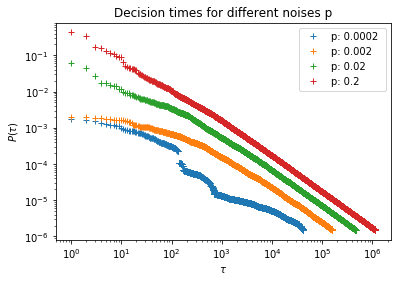
\includegraphics[scale=0.6]{decisionProbas.png}
    \caption{The different decision times for the noises $p$ used in Sznajd's paper. \newline
    Note that we get some of the same effect, however to a lesser extent, in opposite order. I believe the ordering comes from a scaling I do since I got a pretty weird decision times plot without it.}
    \label{fig6}
\end{figure} \newline
This looks a bit off, we see that it does still follow a set of power laws, although different ones.\newpage
\section{Discussion}
\subsection{Similarities and Differences. Comparing to Sznajd}
We were asked to compare our results to the ones found in Sznajd's paper, so lets do that here. \newline
Most of our results are in line with what we find in the paper. The only real outliers are perhaps the decision time plots an any results pertaining to them. While we do see much the same behavior, that is, an increase in density as we move alongside the x-axis, this is simply a result of the plot being logarithmic. What we would've liked to see was a larger spread of values as we continued along the x-axis. An alternative approach I tried yieled somewhat similar results, with a spread at the bottom like so:
\begin{figure}[ht!]
    \centering
    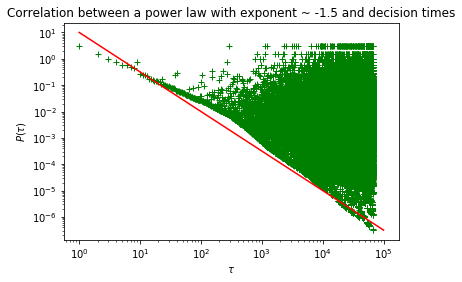
\includegraphics[scale=0.6]{alternativedecisiontimes.png}
    \caption{Using an alternative measure of decision times. \newline
    To me, this one intuitively makes that the counterpart used above in the results, but the plots this gives are so unreadable that I decided not to use it. \newline
    While the plots in the report use the object.adt array to plot, this figure uses object.dt.}
    \label{fig7}
\end{figure} \newline
As seen above, this alternative method does yield a spread at the bottom, but only above the line, which is not what we want. \newline
Other than that we can see that our results are much in line with what else is shown in Sznajd's paper, albeit with some small differences. It is worth noting however, that due to the random nature of this project and algorithm, it is hard to say for certain, especially since the results we can see in Sznajd are limited and the source code is gone (which means we can't take more samples to compare to). \newline
For example, I found it pretty odd that they were able to reach a consensus using only 50000 MCS with 1000 spins, while I have to use upwards of 10 000 000 MCS for 500 spins, and even then there is sometimes never a convergence. \newline
It is also worth noting that I've neglected to include Sznajd's figure 5, because I thought this was pretty obvious and because of the doubts mentioned above. If I were to do 1000 samples of 10 000 000 MCS it'd simply take too long, so apologies.
\section{Conclusion}
In conclusion, we've shown how to model the opinion dynamics of an election with a simple one dimensional Ising Model. We've shown additionally how the decision times for such a model are very commonly small, just like the empirical data shown in \cite{sznajd}'s figure 3. Lastly we've examined different modifications and adjustments to our model like concentrations and noise, and found the effects these have on both the ability to reach a consensus and the relation with the characteristic power law of $-3/2$ for an unmodified model. We then find that our model needs an openness of $p \geq 3\times 10^{-5}$ to avoid a "one-party state".
\bibliographystyle{unsrturl}
\bibliography{citations.bib}

\end{document}
